\section{Supplementary: Method Derivations and Defense-in-Depth Audits}
\label{sec:suppl:method}

This supplementary atom contains the material removed from \S\ref{sec:method} for the CVPR 8-page main paper. The derivations and audits below are the source of the claims that the main paper carries as one-line summaries.

\subsection{Bounded-activation constants and training-configuration hyperparameters}
\label{sec:suppl:method:constants}
Exact constants compressed from \S\ref{sec:method} for the CVPR 8-pp main. \textbf{Bounded physics layer ([D-02]).} Final-layer activations enforce physical scales field-by-field: $\rho/\bar\rho$ via unscaled Softplus, $T$ via $\texttt{Softplus}\cdot 10^4 + 10^3$ K, $X_{HI}$ via Sigmoid in $[0,1]$, and $v_{\text{pec}}$ via $\texttt{Tanh}\cdot 500$ km/s. \textbf{Training configuration ([D-14]/[D-23]).} We optimize with AdamW ($\beta=(0.9,0.999)$, weight decay $10^{-6}$, gradient L2 clip $1.0$) on a single \texttt{ml.g5.xlarge} (NVIDIA A10G, 24 GB) per tier under the tier-aware schedule T1 $n_{\text{rays}}{=}64\,/\,50$k steps, T2 $256/25$k, T3 $1024/12.5$k, T4 $16{,}384/12.5$k (deferred), with per-tier linear-warmup-then-cosine LR $0\!\to\!5\!\times\!10^{-4}\!\to\!5\!\times\!10^{-6}$. Peak VRAM follows the [D-23] linear model $\hat{V}_{\text{peak}}\approx\TonePeakVRAM\cdot\min(n_{\text{rays}},\mu\text{batch})/64$ GB (Tab.~\ref{tab:per-tier-vram}).

\subsection{Saturated-absorber detection: Bolton--Haehnelt derivation}
\label{sec:suppl:method:bh}
Per-sightline, we flag bins with $\tau_{GT} > 10^5$ as saturated cores, then expand each core to its connected component of bins with $\tau_{GT} > 10$ (the saturated wing). The threshold $\tau_{\text{core}} = 10^5$ is derived from the Voigt line-center identity (Bolton \& Haehnelt~\cite{bolton_haehnelt2007} Eq. 5) for thermal Doppler broadening at $T = 10^4$ K:
\begin{equation}
\tau_0 \approx 5.2 \times 10^{-14} \cdot (T/10^4\,\text{K})^{-1/2} \cdot (N_{HI}/\text{cm}^{-2})
\end{equation}
which gives $\tau_0 > 10^5 \Leftrightarrow N_{HI} > \NHIcoreThreshold$ cm$^{-2}$. The threshold sits an order of magnitude below the canonical DLA boundary $N_{HI} \geq \NHIdla$ cm$^{-2}$~\cite{wolfe2005} and includes strong Lyman-limit systems at $N_{HI} \gtrsim \NHIlls$ cm$^{-2}$~\cite{prochaska2010}, so the mask is operationally conservative in the inclusion direction. Detection happens once per sightline at load time and is recorded as a per-bin sidecar mask carried through the loss reduction.

\subsection{Forest cap calibration}
\label{sec:suppl:method:cap}
Surviving non-saturated bins are clipped at $\tau_{\max} = 10$ on both prediction and target before the loss is evaluated. The cap is calibrated on two grounds. First, the flux-PDF gate evaluates KS distance on $F = e^{-\tau}$ over $F \in [\PDFwinLo, \PDFwinHi]$, i.e., $\tau \in [0.051, 3.0]$; capping at $\tau_{\max} = 10$ ($F = e^{-10} \approx 4.5 \times 10^{-5}$) places the cap an order of magnitude above the science measurement range, so it does not bias the gate. Second, for strong-but-non-saturated absorbers ($\tau \in (3, 10]$), the cap bounds the gradient amplitude from the Lorentzian wing, where raw-$\tau$ MSE has non-Gaussian tail behavior that destabilizes optimization. The cap value is locked by the sensitivity gate of Sec.~\ref{sec:suppl:exp:tau-max-sensitivity}.

\subsection{Log-space supervision: [D-38] defense-in-depth argument}
\label{sec:suppl:method:logspace}
The $\log(1+\tau)$ supervision space is the methods contribution of this work, defended on physical rather than NN-precedent grounds. Lyman-alpha-forest opacity is approximately log-normally distributed in $\tau$ across the cool diffuse IGM~\cite{bi_davidsen1997, hui_gnedin1997} as a consequence of the Fluctuating Gunn-Peterson Approximation $\tau \propto \rho^{1.6} T^{-0.7}$ acting on a near-log-normal density PDF; supervising in $\log(1+\tau)$ matches this natural noise model. The $\log(1+\cdot)$ form reduces to $\tau$ in the optically thin limit and is monotone with $-\log F$ for $\tau \gtrsim 1$, so the data loss and the mean-flux anchor pull on the network in compatible spaces. The mask and the cap are not part of this novelty claim; their role is defense-in-depth retained against the rare initialization-stress regimes (e.g., the Physics-2 Tier-3 seed-0 softplus-saturation collapse documented in our cost-survey forensic). The four-cell ablation of Tab.~\ref{tab:s5s7-ablation} shows that on the tested configuration the cap and mask are not load-bearing for convergence to the achieved loss floor; we report this null result as such (per the [D-37] honest-reporting rule) and retain the safeguards for the stressed configurations on which the ablation was not exercised.

\begin{table}[t]
    \centering
    \renewcommand{\arraystretch}{1.15}
    \setlength{\tabcolsep}{4pt}
    \begin{tabular}{l|cccc}
    metric & A: full & B: no-cap & C: no-mask & D: no-cap-no-mask \\
    \hline
    \texttt{loss}        & 0.0052      & 0.0052      & 0.0052      & 0.0052      \\
    \texttt{loss\_data}  & 0.0026      & 0.0026      & 0.0026      & 0.0026      \\
    \texttt{meanF} term  & $2.6203\!\times\!10^{-3}$ & $2.6205\!\times\!10^{-3}$ & $2.6201\!\times\!10^{-3}$ & $2.6203\!\times\!10^{-3}$ \\
    $\langle F\rangle$   & 0.9282      & 0.9282      & 0.9282      & 0.9282      \\
    \texttt{tau\_amp}    & 0.9983      & 1.0026      & 1.0003      & 1.0030      \\
    \end{tabular}
    \caption{\textbf{S5/S7 ablation on the [D-24] loss bundle.} Configuration: Physics-1 (``no feedback''), Tier-2 ($n_{\text{rays}}=256$), seed $=1$, 25k steps; broken anchor $\langle F\rangle_{\text{obs}}=0.877$ (apples-to-apples with the published P1-T2 baseline). All four cells converge to indistinguishable final states on \texttt{loss / loss\_data / meanF / $\langle F\rangle$} (four-decimal identity); only \texttt{tau\_amp} differs by $\leq 0.5\%$, in the calibration-degeneracy direction the [D-11] anchor sub-clause marks uninterpretable. \textbf{Verdict:} the cap and mask are not load-bearing for convergence on this configuration. They are retained as defense-in-depth against initialization-stress regimes; their necessity on stressed configurations is \emph{not} tested by this ablation. \textbf{MLflow run\_ids:} \texttt{ca5a9ff1\dots} (full), \texttt{e563b72a\dots} (no-cap), \texttt{d691268c\dots} (no-mask), \texttt{fce098d3\dots} (no-cap-no-mask).}
    \label{tab:s5s7-ablation}
\end{table}

\begin{figure}[h]
    \centering
    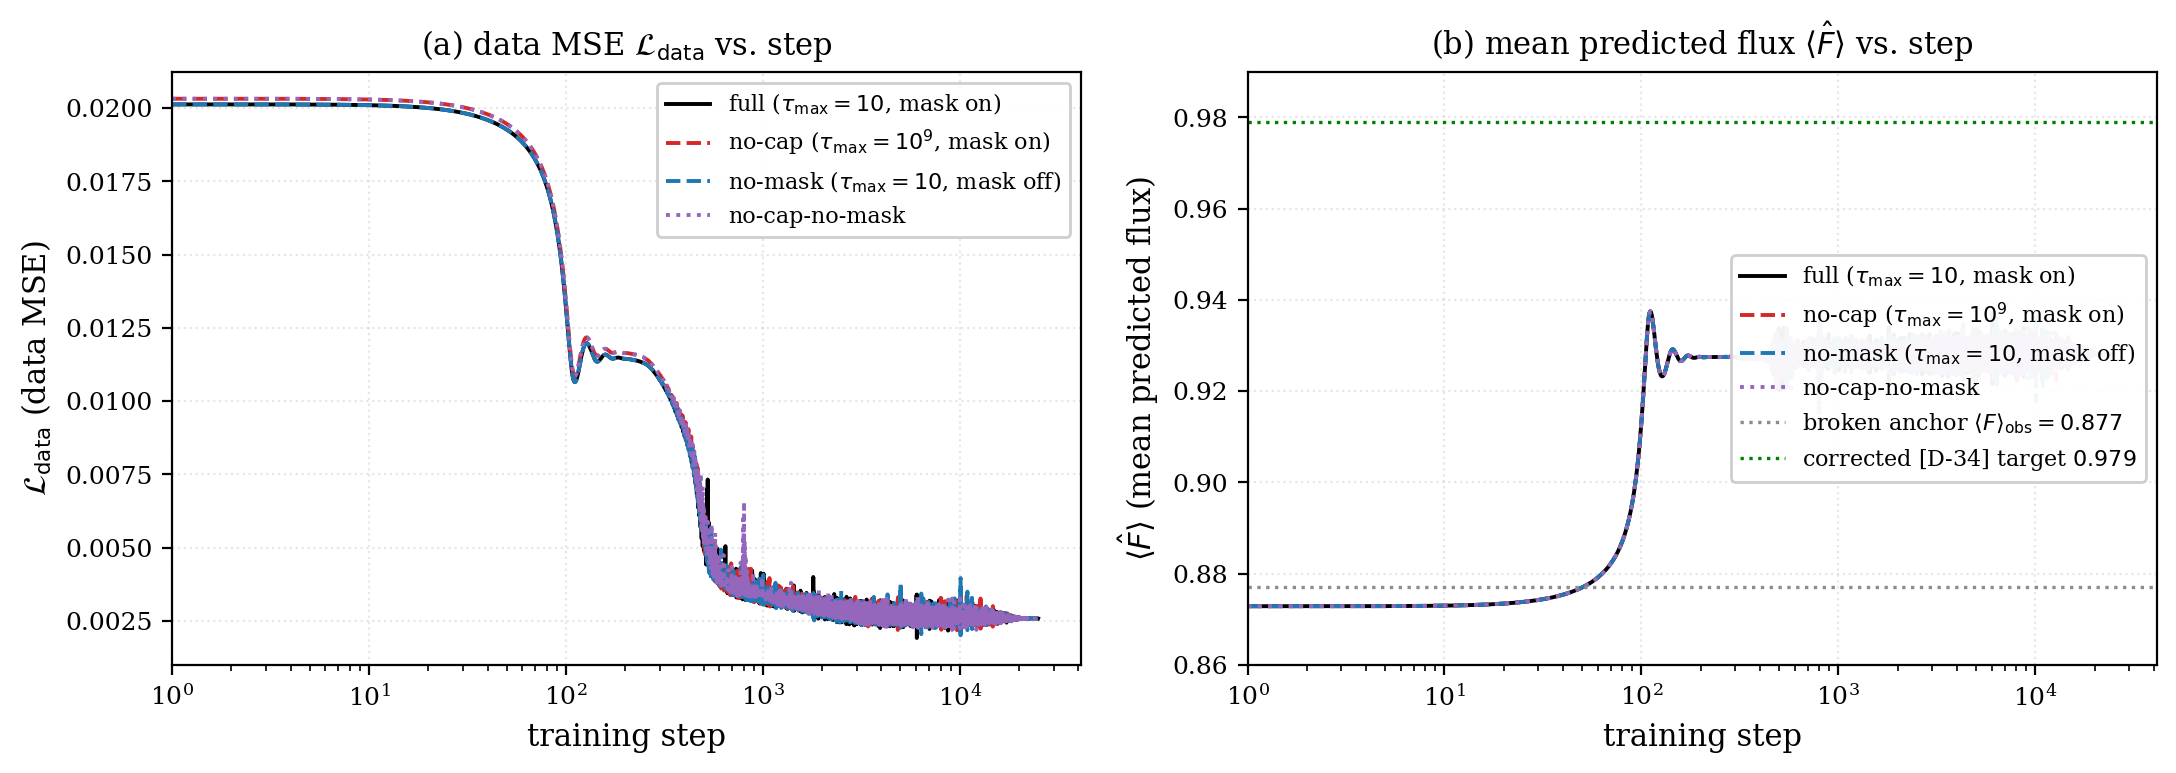
\includegraphics[width=\linewidth]{figures/s5s7_loss_curves.png}
    \caption{\textbf{S5/S7 ablation: training trajectories on T2-P1 seed=1, 25k steps, broken anchor $\langle F\rangle_{\text{obs}}=0.877$.} Left: data MSE $\mathcal{L}_{\text{data}}$ vs.\ step. Right: mean predicted flux $\langle\hat F\rangle$ vs.\ step (with the broken-anchor target 0.877 in gray and the corrected [D-34] target \AnchorMeanF\ in green; the model converges to $\langle\hat F\rangle\approx 0.9282$, between the two). All four cells converge to the same final regime ($\mathcal{L}_{\text{data}}=0.0026$, $\langle\hat F\rangle=0.9282$). The largest inter-cell divergence is at step~1: cells with the cap off (no-cap, no-cap-no-mask) start at $\mathcal{L}_{\text{data}}\approx 0.0203$ vs.\ $\approx 0.0201$ for cap-on cells, a $\sim 1\%$ relative gap that closes by step $\sim 100$ and is below line-width thereafter. \textbf{Verdict:} the cap and mask are not load-bearing on this configuration; they are retained as defense-in-depth ([D-38]).}
    \label{fig:s5s7-loss-curves}
\end{figure}

\subsection{Mean-flux mask consistency and two-pass linearization (proof)}
\label{sec:suppl:method:twopass}
\textbf{Mask consistency.} The mean-flux reduction $\langle e^{-\tau_{\text{pred}}}\rangle$ and the data loss of Eq.~\ref{eq:data-loss} both apply the same saturated-absorber mask of Sec.~\ref{sec:method:loss}. This is load-bearing: a separately-derived prediction-side mask would be circular (saturation in $\tau_{\text{pred}}$ depends on the trainable parameters), so the per-sightline mask is taken from $\tau_{GT}$ at load time and reused unchanged in both reductions. The data loss and the anchor therefore see identical bin sets and the gradient identity below holds without correction terms for the masking operation.

\textbf{Two-pass linearization (chain-rule identity).} The mean-flux constraint is implemented as a two-pass surrogate to avoid \texttt{retain\_graph} in the microbatch grad-accumulation loop. Pass 1 runs the model under \texttt{torch.no\_grad()} to compute the cycle-mean predicted flux $F_{\text{cycle}}$ over all microbatches; Pass 2 then backpropagates a per-microbatch surrogate
\begin{equation*}
\mathcal{L}_{\text{mb}} = \mathcal{L}_{\text{data,mb}} + c \cdot \langle F\rangle_{\text{mb}}, \quad c = 2 \lambda_F (F_{\text{cycle}} - \langle F\rangle_{\text{obs}})
\end{equation*}
where $c$ is a constant for the cycle. By the chain rule $\partial \mathcal{L}_{\text{meanF}}/\partial \theta = c \cdot \partial F_{\text{cycle}}/\partial \theta$ and $\partial F_{\text{cycle}}/\partial \theta = (1/N_{\text{chunks}}) \sum_i \partial \langle F\rangle_{\text{mb},i}/\partial \theta$, so the surrogate's gradient is mathematically identical to the squared-loss gradient at the current parameter point. Re-linearization happens every optimizer step. Memory peak is one microbatch instead of \texttt{accum\_steps} microbatches.

\subsection{Per-tier microbatch and VRAM table}
\label{sec:suppl:method:vram}
\begin{table}[t]
    \centering
    \renewcommand{\arraystretch}{1.15}
    \begin{tabular}{c|c|c|c|c}
    Tier & $n_{\text{rays}}$ & chunk & accum & peak VRAM (GB) \\
    \hline
    T1 & 64    & 64  & 1  & \TonePeakVRAMcell  \\
    T2 & 256   & 256 & 1  & \TtwoPeakVRAMcell \\
    T3 & 1024  & 256 & 4  & \TthreePeakVRAM \\
    T4 & 16384 & 256 & 64 & \TfourPeakVRAM \\
    \end{tabular}
    \caption{Stage 2b micro-grid per-tier peak VRAM measurements, validating the $\hat{V}_{\text{peak}} \approx \TonePeakVRAM \cdot \min(n_{\text{rays}}, \mu\text{batch}) / 64$ GB scaling from [D-23]. All tiers fit $\geq \VRAMHeadroomPercent$ under the 24 GB device VRAM budget; the linear model holds across the full $\text{accum\_steps} \in \{1, 4, 64\}$ range exercised by the production schedule.}
    \label{tab:per-tier-vram}
\end{table}
Microbatch values for tiers 3 and 4 are constrained by VRAM rather than convergence: the per-step chunk size is $\min(n_{\text{rays}}, \mu\text{batch})$, so chunk-size 256 saturates the linear-VRAM budget derived from the tier-1 measurement ($\TonePeakVRAM$ GB at 64 rays). The measured peaks (Tab.~\ref{tab:per-tier-vram}) sit $\geq \VRAMHeadroomPercent$ under the 24 GB device budget across $\text{accum\_steps} \in \{1, 4, 64\}$. Checkpoints sync to S3 every 5{,}000 steps. Tier 4 is deferred to post-quota because its 64-chunk gradient accumulation makes its wallclock per cell dominate the survey budget; tiers 1--3 already span the survey-realistic sightline-density regime. Cost-survey runs are calibration evidence only; publication runs (post-quota) re-run the corresponding tier under the locked-in schedule.
